% =============================================================================
\bloco{2}{Harder: equilibrium, endogenous saving, and the golden rule}{Kurlat \S\S9.1--9.3; Romer \S2.9--2.11 \,\textbullet\, 37 points}

\questao{(6 points) \textit{Source: Kurlat, P. (2020), \emph{A Course in Modern Macroeconomics}, Exercise 9.2 ``Storage'',
pp.~179--180 --- statement reproduced verbatim, all items (a)--(c).}
\emph{What this trains:} prices come from the firm's FOCs and the no-arbitrage condition $1+r=r^K+1-\delta$; the Euler equation then
signs the consumption path.}

\noindent Suppose the production function is the following:
\[
F(K,L)=K
\]
and the rate of depreciation is $\delta=1$.
\begin{enumerate}[label=(\alph*),leftmargin=2.2em,topsep=2pt,itemsep=1pt]
\item Why is this production function called ``storage''?
\item What will be the real interest rate and the wage in this economy?
\item With standard preferences, will consumption increase over time, remain constant over time or decrease over time?
\end{enumerate}
\resolespaco
\begin{sol}
\begin{notacao}
\item $F(K,L)$: production function; $F_K$, $F_L$: marginal products of capital and labour. $\delta\in[0,1]$: depreciation rate.
\item $r^K$: rental rate of capital. $w$: wage. $r$: interest rate.
\item $c_t>0$: consumption at $t$. $u$: utility, $u'>0$, $u''<0$. $\beta\in(0,1)$: discount factor; $\rho\equiv1/\beta-1>0$.
\end{notacao}
\passo{(a)}{One unit of goods put aside as capital today returns exactly one unit tomorrow and then disappears; labour is useless:}
\begin{equation}
F_K=1,\qquad F_L=0,\qquad \delta=1. \label{q5:tech}
\end{equation}
The technology only moves goods through time.
\passo{(b)}{The firm's FOCs set each factor price equal to its marginal product:}
\begin{equation}
r^K=F_K,\qquad w=F_L. \label{q5:foc}
\end{equation}
Substituting \eqref{q5:tech} into \eqref{q5:foc}: $r^K=1$ and $w=0$. No arbitrage between capital and loans, Kurlat (9.3.11):
\begin{equation}
1+r=r^K+1-\delta. \label{q5:arb}
\end{equation}
Substitute $r^K=1$ and $\delta=1$ from \eqref{q5:tech} into \eqref{q5:arb}:
\[
1+r=(1)+1-(1)=1,\qquad r=0 .
\]
Both prices are fixed by the linear technology, whatever $K$ is.
\passo{(c)}{The household's Euler equation:}
\begin{equation}
u'(c_t)=\beta(1+r)u'(c_{t+1}). \label{q5:euler}
\end{equation}
Substitute $r=0$ from (b) into \eqref{q5:euler}:
\begin{align*}
u'(c_t) &= \beta\big(1+(0)\big)u'(c_{t+1})\\
&= \beta u'(c_{t+1}).
\end{align*}
As $\beta<1$, $u'(c_t)<u'(c_{t+1})$ and, $u'$ being decreasing, $c_{t+1}<c_t$: consumption falls over time. A steady state would need
\begin{equation}
F_K-\delta=\rho>0 \label{q5:ss}
\end{equation}
(Kurlat (9.3.17)), but by \eqref{q5:tech} $F_K-\delta=0$ always, so \eqref{q5:ss} never holds.
\intuicao{The return on waiting ($r=0$) is below the rate of time preference ($\rho>0$), so the household runs the warehouse down.}
\refbib{Kurlat (2020), \S9.1, eqs.\ (9.1.9)--(9.1.11); \S9.3, eqs.\ (9.3.11), (9.3.17); project solution \texttt{Resolucao/}\allowbreak\texttt{kurlat\_solutions\_ch09.tex}, Problem 9.2.}
\rubrica{
\item (b) $w$, $r^K$ and $r$ via no arbitrage: 3 pts; $r=1$ (forgetting $\delta$): max.\ 1 pt for (b).
\item (c) Euler and sign: 2 pts. (a): 1 pt.
}
\end{sol}

% -----------------------------------------------------------------------------
\questao{(12 points) \textit{Source: Kurlat, P. (2020), \emph{A Course in Modern Macroeconomics}, Exercises 9.11 ``Patience and
Investment'', p.~185, and 9.12 ``Optimal vs Fixed Savings Rates'', pp.~185--186 (the key synthesis) --- statements reproduced verbatim,
all items. Change: 9.12 is worked in Python (the book points to Matlab code); item (f) is added by this list.}
\emph{What this trains:} the saving rate Solow assumes is the one the optimising economy chooses in the long run; it is below $s_{GR}$.}

\noindent\textit{Added (not in the book): work 9.11 symbolically, and 9.12 in Python (the book points to Matlab code).}\par

\noindent\textbf{9.11 Patience and Investment}\par\noindent Suppose the production function is $F(K,L)=K^\alpha L^{1-\alpha}$, and the labor supply
is exogenous and equal to $L=1$. The representative household's preferences are given by:
\[
\sum_{t=0}^{\infty}\beta^t\frac{c_t^{1-\sigma}}{1-\sigma}
\]
and the depreciation rate is $\delta$.
\begin{enumerate}[label=(\alph*),leftmargin=2.2em,topsep=2pt,itemsep=1pt]
\item Use equation (9.3.17) to find an expression for the level of capital that this economy will have in the steady state.
\item Find an expression for the level of GDP that the economy will have in the steady state.
\item Find an expression for the steady-state investment-to-GDP ratio. How does it depend on $\beta$? Explain.
\end{enumerate}

\noindent\textbf{9.12 Optimal vs Fixed Savings Rates}\par\noindent Suppose the economy is as in Exercise 9.11, with $\alpha=0.4$, $\beta=0.95$, $\delta=0.08$
and $\sigma=2$. The economy starts with an initial capital stock $K_0=2$. We are going to compare how this economy behaves under a
fixed investment rate and under an optimally-chosen investment rate.
\begin{enumerate}[label=(\alph*),leftmargin=2.2em,topsep=2pt,itemsep=1pt]
\item First suppose that, like we assumed in Chapter 4, the investment rate is exogenous and constant, and equal to the steady-state
investment-to-GDP ratio that you found in Exercise 9.11. Compute GDP, consumption, investment and the capital stock for the first
150 years of this economy.
\item Now suppose that consumption and investment are chosen in accordance with (9.3.13). Find the level of initial consumption that
is consistent with the system of equations (9.3.15) - (9.3.13) and the economy converging to a steady state. (You can find a Matlab
code that will compute this at the book website). Compute GDP, consumption, investment and the capital stock for the first 150
years of this economy.
\item Plot the consumption paths of the two economies over the first 150 years on the same graph.
\item Replace the computed paths of consumption from parts (a) and (b) into the utility function to compute how much utility the
representative household will obtain in the first 150 years of each economy.
\item By what fraction would one have to reduce consumption in the optimal-savings economy for the household to get the same utility
as in the exogenous-savings economy?
\end{enumerate}

\noindent\textit{Added parts (not in the book):}\par\nopagebreak
\textbf{(f)} Compare the steady-state investment rate with the golden-rule rate and the steady-state capital with $K_{GR}$.
\resolespaco
\begin{sol}
\begin{notacao}
\item $K_t$: capital (labour is fixed at 1), $Y_t=K_t^\alpha$: output, $\alpha\in(0,1)$. $I_t$: investment. $c_t>0$: consumption.
\item $\delta\in(0,1)$: depreciation. $\beta\in(0,1)$: discount factor; $\rho\equiv1/\beta-1>0$. $\sigma>0$: CRRA curvature,
$u(c)=\frac{c^{1-\sigma}}{1-\sigma}$. $r_t$: interest rate.
\item $K_{SS}$, $Y_{SS}$, $c_{SS}$: steady-state values. $s\equiv I/Y$: investment (saving) rate. $K_{GR}$, $s_{GR}$: golden-rule
capital and saving rate.
\item 9.12: $\alpha=0.4$, $\beta=0.95$, $\delta=0.08$, $\sigma=2$, $K_0=2$, $t=0,\dots,149$. $U$: discounted utility of a path.
$\lambda>0$: the factor that scales a whole consumption path.
\end{notacao}
\passo{9.11(a)}{The steady-state condition, Kurlat (9.3.17), with $F_K=\alpha K^{\alpha-1}$:}
\begin{equation}
\alpha K_{SS}^{\alpha-1}-\delta=\frac1\beta-1=\rho. \label{q6:mgr}
\end{equation}
Add $\delta$ to \eqref{q6:mgr} and divide by $\alpha$:
\[
K_{SS}^{\alpha-1}=\frac{\rho+\delta}\alpha .
\]
Raise both sides to the power $\frac{1}{\alpha-1}$:
\begin{equation}
K_{SS}=\left(\frac{\alpha}{\rho+\delta}\right)^{\frac1{1-\alpha}}. \label{q6:Kss}
\end{equation}
$\sigma$ does not appear.
\passo{9.11(b)}{Raise \eqref{q6:Kss} to the power $\alpha$:}
\begin{align}
Y_{SS}=K_{SS}^\alpha &= \left[\left(\frac{\alpha}{\rho+\delta}\right)^{\frac1{1-\alpha}}\right]^{\alpha}\nonumber\\
&= \left(\frac{\alpha}{\rho+\delta}\right)^{\frac{\alpha}{1-\alpha}}, \label{q6:Yss}
\end{align}
increasing in $\beta$ (higher $\beta$, lower $\rho$).
\passo{9.11(c)}{In the steady state investment only replaces depreciation:}
\begin{equation}
I=\delta K_{SS}. \label{q6:I}
\end{equation}
Divide \eqref{q6:I} by $Y_{SS}=K_{SS}^\alpha$, then use \eqref{q6:Kss}:
\begin{align}
\frac IY &= \frac{(\delta K_{SS})}{(K_{SS}^\alpha)}\nonumber\\
&= \delta K_{SS}^{1-\alpha}\nonumber\\
&= \delta\left[\left(\frac{\alpha}{\rho+\delta}\right)^{\frac1{1-\alpha}}\right]^{1-\alpha}\nonumber\\
&= \frac{\alpha\delta}{\rho+\delta}. \label{q6:IY}
\end{align}
\passo{9.12 numbers}{With $\alpha=0.4$, $\beta=0.95$, $\delta=0.08$:}
\begin{align*}
\rho &= 1/0.95-1=0.052632,\qquad \rho+\delta=0.132632,\qquad \alpha/(\rho+\delta)=3.015873,\\
K_{SS} &= 3.015873^{1/0.6}=6.2954 &&\text{by \eqref{q6:Kss}},\\
Y_{SS} &= 6.2954^{0.4}=2.0874 &&\text{by \eqref{q6:Yss}},\\
s &\equiv I/Y=(0.4)(0.08)/0.132632=0.241270 &&\text{by \eqref{q6:IY}},\\
c_{SS} &= Y_{SS}-\delta K_{SS}=2.0874-(0.08)(6.2954)=1.5838 &&\text{by \eqref{q6:I}}.
\end{align*}
\passo{9.12(a)}{The fixed-rate economy, with $1-\delta=0.92$:}
\begin{equation}
Y_t=K_t^{0.4},\quad I_t=sY_t,\quad c_t=(1-s)Y_t,\quad K_{t+1}=0.92K_t+I_t. \label{q6:fixed}
\end{equation}
Iterate \eqref{q6:fixed} from $K_0=2$:
\begin{align*}
Y_0 &= 2^{0.4}=1.3195,\\
c_0 &= 0.758730\times1.3195=1.0012,\\
I_0 &= 0.241270\times1.3195=0.3184,\\
K_1 &= 0.92\times2+0.3184=2.1584.
\end{align*}
\passo{9.12(b)}{The optimal economy obeys the resource constraint and the Euler equation. With CRRA utility the Euler equation is
$c_{t+1}=c_t[\beta(1+r_{t+1})]^{1/\sigma}$, and by no arbitrage $1+r_{t+1}=\alpha K_{t+1}^{\alpha-1}+1-\delta$. Substituting the
no-arbitrage rate into the Euler equation, then the parameters:}
\begin{align}
K_{t+1} &= 0.92K_t+K_t^{0.4}-c_t, \label{q6:res}\\
c_{t+1} &= c_t\big[\beta\big(\alpha K_{t+1}^{\alpha-1}+1-\delta\big)\big]^{1/\sigma}\nonumber\\
&= c_t\big[0.95(1+0.4K_{t+1}^{-0.6}-0.08)\big]^{1/2}. \label{q6:eul}
\end{align}
Iterate \eqref{q6:res}--\eqref{q6:eul} from a guess $c_0$; bisect: if $K$ overshoots $K_{SS}$, raise $c_0$; if $c$ starts falling (or $K$
turns down) before $K_{SS}$, lower $c_0$. The saddle path gives $c_0=0.920627$. Then, by \eqref{q6:res}:
\[
I_0=1.3195-0.9206=0.3989,\qquad K_1=0.92\times2+0.3989=2.2389 .
\]
\passo{9.12(c)}{Selected years (both economies start at $K_0=2$ and end at the same steady state):}
\begin{center}\small\begin{tabular}{rrrrrrr}\toprule
$t$ & $K$ fixed & $K$ optimal & $c$ fixed & $c$ optimal & $I$ fixed & $I$ optimal\\\midrule
0 & 2.0000 & 2.0000 & 1.0012 & 0.9206 & 0.3184 & 0.3989\\
5 & 2.7603 & 3.1169 & 1.1389 & 1.1297 & 0.3622 & 0.4461\\
10 & 3.4262 & 4.0048 & 1.2417 & 1.2719 & 0.3948 & 0.4701\\
25 & 4.8324 & 5.4958 & 1.4248 & 1.4818 & 0.4531 & 0.4953\\
50 & 5.8509 & 6.1667 & 1.5381 & 1.5678 & 0.4891 & 0.5025\\
149 & 6.2919 & 6.2954 & 1.5834 & 1.5838 & 0.5035 & 0.5036\\\bottomrule
\end{tabular}\end{center}
\begin{center}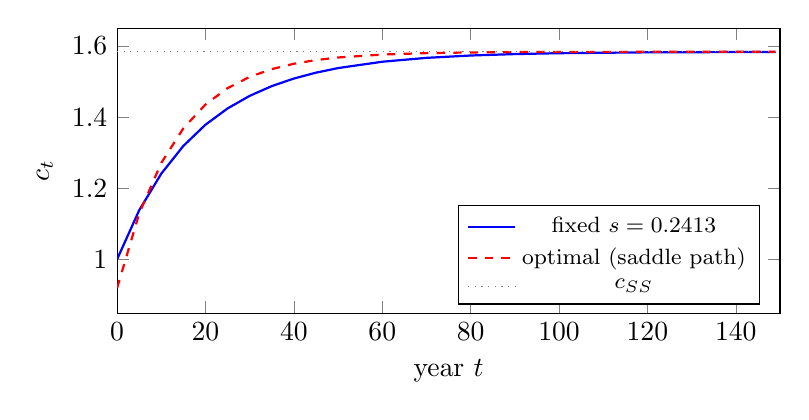
\begin{tikzpicture}\begin{axis}[width=10cm,height=5.2cm,xlabel={year $t$},ylabel={$c_t$},legend pos=south east,
legend style={font=\footnotesize},xmin=0,xmax=150,ymin=0.85,ymax=1.65]
\addplot[blue,thick] coordinates {(0,1.0012) (5,1.1389) (10,1.2417) (15,1.3196) (20,1.3791) (25,1.4248) (30,1.4601) (35,1.4875) (40,1.5087) (45,1.5252) (50,1.5381) (60,1.5559) (70,1.5668) (80,1.5734) (90,1.5774) (100,1.5799) (120,1.5823) (149,1.5834)};
\addplot[red,thick,dashed] coordinates {(0,0.9206) (5,1.1297) (10,1.2719) (15,1.3691) (20,1.4359) (25,1.4818) (30,1.5134) (35,1.5352) (40,1.5502) (45,1.5606) (50,1.5678) (60,1.5761) (70,1.5801) (80,1.5820) (90,1.5830) (100,1.5834) (120,1.5837) (149,1.5838)};
\addplot[gray,dotted] coordinates {(0,1.5838) (150,1.5838)};
\legend{fixed $s=0.2413$, optimal (saddle path), $c_{SS}$}
\end{axis}\end{tikzpicture}\end{center}
The optimal economy consumes less at first and more later; the paths cross between years 5 and 6.
\passo{9.12(d)}{With $\sigma=2$, $u(c)=\frac{c^{-1}}{-1}=-1/c$. Discounted utility of a path:}
\begin{equation}
U=\sum_{t=0}^{149}0.95^t u(c_t). \label{q6:U}
\end{equation}
Evaluating \eqref{q6:U} on the two paths of (c):
\[
U^{\text{fixed}}=-15.79988,\qquad U^{\text{opt}}=-15.74360 ;
\]
the optimal path is better.
\passo{9.12(e)}{Scaling every $c_t$ by $\lambda$ multiplies each $u(c_t)$ in \eqref{q6:U}, and so $U$, by $\lambda^{1-\sigma}$:}
\begin{equation}
U(\lambda c)=\lambda^{1-\sigma}U(c)=\lambda^{-1}U(c). \label{q6:scale}
\end{equation}
Using \eqref{q6:scale}, solve $\lambda^{-1}U^{\text{opt}}=U^{\text{fixed}}$:
\[
\lambda=\frac{U^{\text{opt}}}{U^{\text{fixed}}}=\frac{(-15.74360)}{(-15.79988)}=0.996438,
\]
a cut of $1-\lambda=0.356\%$ of consumption.
\passo{(f) golden rule}{$s=0.2413<s_{GR}=\alpha=0.40$. Rewrite \eqref{q6:IY}:}
\[
\frac IY=\alpha\cdot\frac{\delta}{\rho+\delta},\qquad \frac{\delta}{\rho+\delta}<1\iff\rho>0 .
\]
$K_{GR}$ maximises steady-state consumption $K^\alpha-\delta K$, so it solves
\begin{equation}
F_K=\alpha K_{GR}^{\alpha-1}=\delta. \label{q6:gr}
\end{equation}
Solve \eqref{q6:gr} as in 9.11(a):
\[
K_{GR}=(\alpha/\delta)^{\frac1{1-\alpha}}=\big((0.4)/(0.08)\big)^{\frac1{1-(0.4)}}=5^{1/0.6}=14.62>K_{SS}=6.30 .
\]
Comparing \eqref{q6:gr} with \eqref{q6:mgr}, the gap closes only as $\beta\to1$ ($\rho\to0$).
\intuicao{The right constant saving rate costs only a third of a percent of consumption: Solow's assumption is cheap when $s$ is the
equilibrium's long-run rate. That rate is set by impatience, not by the golden rule.}
\refbib{Kurlat (2020), \S9.3, eqs.\ (9.3.13)--(9.3.17), pp.~172--178; \S4.3, eq.\ (4.3.4). Numbers match the project's solution
\texttt{Resolucao/}\allowbreak\texttt{kurlat\_solutions\_ch09.tex}, Problems 9.11--9.12 ($c_0=0.9206271904$, $\lambda=0.996438$). The instructor's PSET~5 covers
the Euler equation and arbitrage of the same economy (Lista 5, Q2) but stops before the steady state.}
\rubrica{
\item 9.11 closed forms: 3 pts. 9.12(a)--(b) with a correct shooting rule: 4 pts; $c_0$ guessed rather than found: max.\ 1 pt for (b).
\item (c)--(e): 3 pts. (f): 2 pts. Ceiling: claiming $K_{SS}=K_{GR}$ ``because of the First Welfare Theorem'': 0 for (f).
}
\end{sol}

% -----------------------------------------------------------------------------
\questao{(9 points) \textit{Source: Romer, D. (2012), \emph{Advanced Macroeconomics}, 4th ed., Problem 2.16 ``Depreciation in the
Diamond model and microeconomic foundations for the Solow model'', p.~97 --- statement reproduced verbatim, all items (a)--(b), preceded
by the set-up and part (a) of Problem 2.15, p.~97, which 2.16(b) refers to (2.15(b)--(d) omitted); item (c) is added by this list.}
\emph{Harder, contrast.} \emph{What this trains:} the exam's ``Solow with $\delta=1$'' remark done right, in
the overlapping-generations reading where the young save only their wage.}

\noindent\textit{Added (not in the book): Problem 2.15 is included because 2.16(b) refers to it.}\par

\noindent\textbf{2.15.} \emph{A discrete-time version of the Solow model.} Suppose $Y_t=F(K_t,A_tL_t)$, with
$F(\bullet)$ having constant returns to scale and the intensive form of the production function satisfying the Inada conditions.
Suppose also that $A_{t+1}=(1+g)A_t$, $L_{t+1}=(1+n)L_t$, and $K_{t+1}=K_t+sY_t-\delta K_t$.
\begin{enumerate}[label=(\alph*),leftmargin=2.2em,topsep=2pt,itemsep=1pt]
\item Find an expression for $k_{t+1}$ as a function of $k_t$.
\end{enumerate}

\noindent\textbf{2.16.} \emph{Depreciation in the Diamond model and microeconomic foundations for the Solow model.} Suppose that in the Diamond model capital depreciates at rate $\delta$, so that $r_t=f'(k_t)-\delta$.
\begin{enumerate}[label=(\alph*),leftmargin=2.2em,topsep=2pt,itemsep=1pt]
\item How, if at all, does this change in the model affect equation (2.59) giving $k_{t+1}$ as a function of $k_t$?
\item In the special case of logarithmic utility, Cobb--Douglas production, and $\delta=1$, what is the equation for $k_{t+1}$ as a
function of $k_t$? Compare this with the analogous expression for the discrete-time version of the Solow model with $\delta=1$ from
part (a) of Problem 2.15.
\end{enumerate}

\noindent\textit{Added parts (not in the book):}\par\nopagebreak
\textbf{(c)} Compare the implied saving rate with $s_{GR}$ and state when this economy over-accumulates.
\resolespaco
\begin{sol}
\begin{notacao}
\item $C_{1t}$, $C_{2t+1}$: consumption of generation $t$ when young and when old. $\rho>-1$: discount rate, $\beta\equiv\frac1{1+\rho}$.
\item $A_t$, $L_t$: technology and number of young, growing at rates $g$ and $n$. $k\equiv K/(AL)$: capital per effective worker;
$f(k)$: intensive production function, $f'>0$, $f''<0$; Cobb--Douglas $f(k)=k^\alpha$, $\alpha\in(0,1)$.
\item $w_t$: wage per effective worker. $r_{t+1}$: interest rate. $\delta\in[0,1]$: depreciation.
\item $s(r)$: share of the wage the young save. $s_S$: Solow's saving rate that reproduces the same law of motion. $s_{GR}$: golden-rule rate.
\end{notacao}
\passo{(a)}{Young at $t$ maximise $\ln C_{1t}+\beta\ln C_{2t+1}$ subject to}
\begin{equation}
C_{1t}+\frac{C_{2t+1}}{1+r_{t+1}}=A_tw_t. \label{q7:pv}
\end{equation}
\eqref{q7:pv} does not contain $\delta$, so the saving rule $s(r_{t+1})$ out of the wage is unchanged by depreciation. Only the return
changes:
\begin{equation}
r_{t+1}=f'(k_{t+1})-\delta. \label{q7:r}
\end{equation}
Market clearing: next period's capital is the young's saving,
\begin{equation}
K_{t+1}=s(r_{t+1})A_tw_tL_t. \label{q7:mc}
\end{equation}
The competitive wage per effective worker is
\begin{equation}
w=f(k)-kf'(k). \label{q7:w}
\end{equation}
Divide \eqref{q7:mc} by $A_{t+1}L_{t+1}=(1+n)(1+g)A_tL_t$, then substitute \eqref{q7:r} and \eqref{q7:w}:
\begin{align}
k_{t+1} &= \frac{s(r_{t+1})A_tw_tL_t}{\big((1+n)(1+g)A_tL_t\big)}\nonumber\\
&= \frac{s(r_{t+1})\,w_t}{(1+n)(1+g)}\nonumber\\
&= \frac{s(f'(k_{t+1})-\delta)\,[f(k_t)-k_tf'(k_t)]}{(1+n)(1+g)}. \label{q7:lom}
\end{align}
In \eqref{q7:lom} depreciation matters only through $s(\cdot)$: in the log case not at all.
\passo{(b)}{Log utility: the young save the share $\frac{\beta}{1+\beta}$ of the wage. Substitute $\beta=\frac1{1+\rho}$:}
\begin{align}
s &= \frac{\big(1/(1+\rho)\big)}{1+\big(1/(1+\rho)\big)}\nonumber\\
&= \frac{1/(1+\rho)}{(2+\rho)/(1+\rho)}\nonumber\\
&= \frac1{2+\rho}, \label{q7:s}
\end{align}
independent of $r$. Cobb--Douglas in \eqref{q7:w}:
\begin{align}
w &= \big(k^\alpha\big)-k\big(\alpha k^{\alpha-1}\big)\nonumber\\
&= k^\alpha-\alpha k^\alpha=(1-\alpha)k^\alpha. \label{q7:wcd}
\end{align}
Substitute \eqref{q7:s} and \eqref{q7:wcd} into \eqref{q7:lom}:
\begin{align}
k_{t+1} &= \frac{\big(\frac1{2+\rho}\big)\big((1-\alpha)k_t^\alpha\big)}{(1+n)(1+g)}\nonumber\\
&= \frac{(1-\alpha)k_t^\alpha}{(2+\rho)(1+n)(1+g)}. \label{q7:lomlog}
\end{align}
Solow 2.15(a) with $\delta=1$:
\begin{equation}
k_{t+1}=\frac{s_Sk_t^\alpha}{(1+n)(1+g)}. \label{q7:solow}
\end{equation}
\eqref{q7:lomlog} and \eqref{q7:solow} are identical with
\begin{align}
s_S &= \frac{1-\alpha}{2+\rho}\nonumber\\
&= \frac{1-\alpha}{2+\big(\frac1\beta-1\big)}\nonumber\\
&= \frac{(1-\alpha)\beta}{1+\beta}: \label{q7:sS}
\end{align}
the young's saving of their wage is the whole gross saving, since with $\delta=1$ the old hold no capital to run down.
\passo{(c)}{Golden rule: $s_{GR}=\alpha$ (Question~2, \eqref{q2:sgr}). Over-accumulation means \eqref{q7:sS} exceeds it. Multiply by
$1+\beta$ and collect terms:}
\begin{align*}
\frac{(1-\alpha)\beta}{1+\beta} &> \alpha\\
\beta-\alpha\beta &> \alpha+\alpha\beta\\
\beta(1-2\alpha) &> \alpha.
\end{align*}
As $\beta<1$, the left side is below $1-2\alpha$, so this needs $1-2\alpha>\alpha$, i.e.\ $\alpha<\frac13$. E.g.\ $\alpha=0.2$, $\beta=0.9$:
\[
s_S=\frac{(1-0.2)(0.9)}{1+(0.9)}=0.8\times0.9/1.9=0.379>0.2 .
\]
Unlike Kurlat's infinite-horizon economy (Q6(f)), finite lives can put the equilibrium above the golden rule.
\intuicao{Diamond microfounds Solow's constant $s$ only in a knife-edge case (log, Cobb--Douglas, $\delta=1$), and the saving rate it
delivers comes from preferences and the wage share, not from any golden-rule calculation.}
\refbib{Romer (2012), \S\S2.9--2.11, eq.\ (2.60), pp.~78--91; Romer, \emph{Solution Manual}, Problems 2.15 and 2.16: same law of motion,
$s(r)=1/(2+\rho)$ and aggregate saving rate $(1-\alpha)/(2+\rho)$. Kurlat (2020), \S9.1 (two-period equilibrium).}
\rubrica{
\item (a) market clearing $K_{t+1}=$ young's saving and the role of $\delta$ through $r$ only: 3 pts.
\item (b) law of motion and the identification $s_S=(1-\alpha)\beta/(1+\beta)$: 4 pts; $s_S=\beta/(1+\beta)$ (forgetting that only wages are saved): max.\ 2 pts.
\item (c): 2 pts.
}
\end{sol}

% -----------------------------------------------------------------------------
\questao{(10 points) \emph{Conceptual, words only.} True or false? Justify each in at most four lines, without algebra.}

\textbf{a)} (2 points) In the exam's economy (log utility over $c_1,c_2$; one unit of time; work carries no disutility; $w_1>0$), no
first-order condition for $L_1$ exists, so $L_1$ is left undetermined.
\gabarito{F}
\begin{sol}
\begin{notacao}
\item $L_1\in[0,1]$: hours worked in period 1. $w_1>0$: wage. $\mathcal L$: the household's Lagrangian.
\item $\lambda>0$: multiplier on the budget (utility value of one unit of resources). $\nu\ge0$: multiplier on $L_1\le1$.
\end{notacao}
\passo{why}{$L_1$ is not in utility but it is in the budget: an extra hour adds $w_1$ to resources, worth $\lambda w_1>0$ in utility. The
marginal gain is positive at every $L_1<1$, so the constraint $L_1\le1$ binds: $L_1=1$, a corner. Stating ``$\partial\mathcal L/\partial L_1=\lambda w_1-\nu=0$
with $\nu>0$, hence $L_1=1$'' \emph{is} the FOC. With leisure in utility it becomes interior (Q9).}
\end{sol}

\textbf{b)} (2 points) With $u=\ln c$ the saving rate does not depend on $r$; so in Kurlat 6.2 a rate cut leaves every person's
$s=(y-c)/y$ unchanged.
\gabarito{F}
\begin{sol}
\begin{notacao}
\item $y_1,y_2\ge0$: income in periods 1 and 2; $c_1$: period-1 consumption; $s=(y-c)/y$: saving out of current income.
\item $r>-1$: interest rate. $\beta\in(0,1)$: discount factor.
\end{notacao}
\passo{why}{Log makes saving a constant share $\frac\beta{1+\beta}$ of \emph{lifetime wealth}, and $c_1$ independent of $r$ only when all resources
arrive in period 1 (the exam). With future income, wealth $y_1+\frac{y_2}{1+r}$ rises when $r$ falls, so $c_1$ rises and $s$ out of current
income falls: strongly for residents, hardly for athletes.}
\end{sol}

\textbf{c)} (2 points) The First Welfare Theorem holds in Kurlat's infinite-horizon economy, so its steady state is the golden rule.
\gabarito{F}
\begin{sol}
\begin{notacao}
\item $F_K$: marginal product of capital. $\delta\in(0,1)$: depreciation. $\rho>0$: rate of time preference.
\item $K_{SS}$: steady-state capital ($F_K=\rho+\delta$); $K_{GR}$: golden-rule capital ($F_K=\delta$).
\end{notacao}
\passo{why}{The golden rule maximises consumption \emph{in the steady state}, ignoring the cost of getting there. Reaching it means giving up
consumption now for gains later, which impatient households value less. Efficiency is relative to their preferences: the modified
golden rule $F_K=\rho+\delta>\delta$ puts $K_{SS}$ below $K_{GR}$. No contradiction.}
\end{sol}

\textbf{d)} (2 points) An economy with capital above the golden rule is dynamically inefficient: a permanently lower saving rate raises
consumption at every date, starting today.
\gabarito{T}
\begin{sol}
\begin{notacao}
\item $s$: saving rate. $k$: capital per (effective) worker; $k_{GR}$: its golden-rule level.
\item $r$: interest rate. $n$, $g$: growth rates of population and technology.
\end{notacao}
\passo{why}{Cutting $s$ raises consumption at once; as capital falls toward $k_{GR}$, steady-state consumption rises (it falls in $k$ above
$k_{GR}$), so no date loses. Equivalently $r<n$ ($+g$). This Pareto improvement cannot exist in Kurlat's economy (Q6(f)) but can in
overlapping generations (Q7(c), Q10), where infinitely many generations break the welfare theorem.}
\end{sol}

\textbf{e)} (2 points) Once the household's rule $a_1=\frac{\beta}{1+\beta}\times$(resources) is known, the economy's law of motion $k_2=\phi(k_1)$
follows without further conditions.
\gabarito{F}
\begin{sol}
\begin{notacao}
\item $a_1$: the household's saving (assets carried to period 2). $k_1$, $k_2$ ($K_1$, $K_2$): capital in periods 1 and 2;
$\phi$: the law of motion $k_2=\phi(k_1)$.
\item $w_1$: wage. $\Pi_1$: profit paid to the household that owns the firm. $Y_1$: period-1 output.
\end{notacao}
\passo{why}{$a_1$ is a demand for assets at given prices. Three more pieces are needed: firm FOCs that turn $k_1$ into $w_1$ and $\Pi_1$
(resources $=Y_1$ when the household owns the firm), market clearing $K_2=a_1$ (capital is the only asset), and the period timing. Only
then is saving a law of motion.}
\end{sol}
\begin{sol}
\rubrica{
\item Each item: 0.5 for the verdict, 1.5 for the reason. A right verdict with a wrong reason: 0.5.
}
\end{sol}
